\documentclass[12pt,a4paper]{article}

% ------------------------------------------------------------
% Encoding, fonts, layout
% ------------------------------------------------------------
\usepackage[T1]{fontenc}
\usepackage[utf8]{inputenc}
\usepackage{lmodern}
\usepackage{microtype}
\usepackage[a4paper,margin=1in]{geometry}
\setlength{\parskip}{0.5em}
\setlength{\parindent}{0pt}

% ------------------------------------------------------------
% Tables, lists, graphics
% ------------------------------------------------------------
\usepackage{array}
\usepackage{booktabs}
\usepackage[table]{xcolor}
\usepackage{adjustbox}
\usepackage{enumitem}
\setlist[itemize]{topsep=4pt,itemsep=2pt,parsep=0pt,partopsep=0pt}
\setlist[enumerate]{topsep=4pt,itemsep=2pt,parsep=0pt,partopsep=0pt}

% ------------------------------------------------------------
% Math
% ------------------------------------------------------------
\usepackage{amsmath,amssymb,amsthm,mathtools}
\allowdisplaybreaks

\DeclareMathOperator{\id}{id}
\DeclareMathOperator{\im}{im}
\DeclareMathOperator{\coker}{coker}
\DeclareMathOperator{\Hom}{Hom}
\DeclareMathOperator{\Spec}{Spec}
\DeclareMathOperator{\Proj}{Proj}
\DeclareMathOperator{\Log}{Log}
\DeclareMathOperator*{\colim}{colim}

\newcommand{\Ab}{\mathbf{Ab}}
\newcommand{\PreSh}{\mathbf{PreSh}}
\newcommand{\Sh}{\mathbf{Sh}}
\newcommand{\AffSch}{\mathbf{AffSch}}
\newcommand{\Sch}{\mathrm{Sch}}
\newcommand{\Rings}{\mathrm{Rings}}

\newcommand{\A}{\mathbb A}
\newcommand{\CC}{\mathbb C}
\newcommand{\GG}{\mathbb G}
\newcommand{\PP}{\mathbb P}
\newcommand{\Pj}{\mathbb P}
\newcommand{\RR}{\mathbb R}
\newcommand{\ZZ}{\mathbb Z}
\newcommand{\Z}{\mathbb Z}

\newcommand{\B}{\mathcal B}
\newcommand{\C}{\mathcal C}
\newcommand{\F}{\mathcal F}
\newcommand{\G}{\mathcal G}
\newcommand{\I}{\mathcal I}
\newcommand{\Ocal}{\mathcal O}
\newcommand{\OO}{\mathcal O}
\newcommand{\OOX}{\mathcal O_X}
\newcommand{\Czero}{\mathcal C^0}
\newcommand{\CzeroX}{\mathcal C^0_X}
\newcommand{\Cinfty}{\mathcal C^\infty}
\newcommand{\CinftyM}{\mathcal C^\infty_M}
\newcommand{\Fp}{\mathcal F'}
\newcommand{\Fpp}{\mathcal F''}

\newcommand{\GammaX}{\Gamma(X,\mathcal O_X)}
\newcommand{\GammaU}[1]{\Gamma(U,#1)}
\newcommand{\kappares}{\kappa}
\newcommand{\nilrad}{\sqrt{(0)}}
\newcommand{\Frac}{\operatorname{Frac}}
\newcommand{\codim}{\operatorname{codim}}
\newcommand{\trdeg}{\operatorname{trdeg}}
\newcommand{\height}{\operatorname{height}}
\newcommand{\Pic}{\operatorname{Pic}}
\newcommand{\divisor}{\operatorname{div}}
\newcommand{\Cl}{\operatorname{Cl}}
\newcommand{\SSone}{S^1}

% ------------------------------------------------------------
% TikZ and diagrams
% ------------------------------------------------------------
\usepackage{tikz}
\usetikzlibrary{arrows.meta,calc,decorations.pathreplacing,fit,positioning,shapes.geometric}
\usepackage{tikz-cd}

% ------------------------------------------------------------
% Links
% ------------------------------------------------------------
\usepackage{hyperref}
\usepackage{bookmark}
\hypersetup{
  colorlinks=true,
  linkcolor=blue!50!black,
  urlcolor=blue!50!black,
  citecolor=blue!50!black,
  pdftitle={Algebraic Geometry 20},
  pdfauthor={},
  pdfsubject={Lecture notes (reorganized)},
  pdfcreator={TeXstudio / LaTeX}
}

% ------------------------------------------------------------
% Theorem environments
% ------------------------------------------------------------
\newtheorem{theorem}{Theorem}[section]
\newtheorem{proposition}[theorem]{Proposition}
\newtheorem{lemma}[theorem]{Lemma}

\newtheoremstyle{notespace}{6pt}{6pt}{\normalfont}{}{\bfseries}{.}{0.5em}{}
\theoremstyle{notespace}
\newtheorem{definition}{Definition}[subsection]
\newtheorem{corollary}[definition]{Corollary}
\newtheorem{remark}[definition]{Remark}
\newtheorem{example}[definition]{Example}
\newtheorem{warning}[definition]{Warning}

% ------------------------------------------------------------
% Section numbering and headers
% ------------------------------------------------------------
\setcounter{tocdepth}{2}
\setcounter{secnumdepth}{2}
\usepackage{fancyhdr}
\pagestyle{fancy}
\fancyhf{}
\lhead{Theory of Algebraic Geometry 22}
\rhead{\thepage}
\renewcommand{\headrulewidth}{0.4pt}
\setlength{\headheight}{14.5pt}


\begin{document}


\title{Algebraic Geometry 22\\
	\large Riemann surfaces}
\author{}
\date{}

	\maketitle
	

	\setcounter{section}{0}

\tableofcontents

	\clearpage

\section{Parallel Transport on the Sphere}

\subsection{The unit sphere and its tangent planes}

Consider the unit sphere embedded in Euclidean space:

\[
S^2
=
\left\{
p\in\mathbb{R}^3:
\langle p,p\rangle=1
\right\}.
\]

Here \(\langle\cdot,\cdot\rangle\) denotes the ordinary Euclidean scalar
product in \(\mathbb{R}^3\).

Let

\[
p\in S^2.
\]

The tangent plane to \(S^2\) at \(p\) is

\[
\boxed{
	T_pS^2
	=
	\left\{
	v\in\mathbb{R}^3:
	\langle p,v\rangle=0
	\right\}.
}
\]

Thus, a tangent vector at \(p\) is perpendicular to the radius vector
from the origin to \(p\).

\subsubsection{Proof}

Let

\[
\alpha:(-\varepsilon,\varepsilon)\longrightarrow S^2
\]

be a smooth curve satisfying

\[
\alpha(0)=p.
\]

Because \(\alpha(s)\in S^2\), we have

\[
\langle\alpha(s),\alpha(s)\rangle=1.
\]

Differentiating with respect to \(s\), we obtain

\[
2\langle\alpha(s),\alpha'(s)\rangle=0.
\]

At \(s=0\),

\[
\langle p,\alpha'(0)\rangle=0.
\]

Since every tangent vector is the velocity vector of some curve through
\(p\), every tangent vector is perpendicular to \(p\). Therefore,

\[
T_pS^2
=
\left\{
v\in\mathbb{R}^3:
\langle p,v\rangle=0
\right\}.
\]

\subsection{Vector fields along curves}

Let

\[
\gamma:[a,b]\longrightarrow S^2
\]

be a smooth curve.

A vector field along \(\gamma\) is a smooth map

\[
V:[a,b]\longrightarrow\mathbb{R}^3
\]

such that

\[
V(t)\in T_{\gamma(t)}S^2
\]

for every \(t\).

Because

\[
T_{\gamma(t)}S^2
=
\left\{
v:
\langle\gamma(t),v\rangle=0
\right\},
\]

the tangency condition is

\[
\boxed{
	\langle\gamma(t),V(t)\rangle=0.
}
\]

Notice that the vectors \(V(t)\) lie in different tangent planes:

\[
V(t_1)\in T_{\gamma(t_1)}S^2,
\qquad
V(t_2)\in T_{\gamma(t_2)}S^2.
\]

They cannot be compared directly as intrinsic tangent vectors. The
ambient space \(\mathbb{R}^3\) allows us to differentiate them and then
project the derivative onto the appropriate tangent plane.

\subsection{The induced Levi--Civita connection}

Let \(W(t)\) be a vector field along \(\gamma\). Its ordinary derivative

\[
\dot W(t)=\frac{dW}{dt}
\]

is a vector in the ambient space \(\mathbb{R}^3\).

In general, \(\dot W(t)\) need not be tangent to the sphere. It can be
decomposed uniquely into tangent and normal components:

\[
\dot W
=
\left(\dot W\right)^{\top}
+
\left(\dot W\right)^{\perp}.
\]

The Levi--Civita derivative along \(\gamma\) is defined by taking the
tangential component:

\[
\boxed{
	\nabla_{\dot\gamma}W
	=
	\operatorname{proj}_{T_{\gamma(t)}S^2}
	\left(\dot W\right).
}
\]

For the unit sphere, the normal direction at \(\gamma(t)\) is generated
by \(\gamma(t)\). Since

\[
\|\gamma(t)\|=1,
\]

the orthogonal projection of a vector \(X\in\mathbb{R}^3\) onto the
tangent plane is

\[
\operatorname{proj}_{T_{\gamma(t)}S^2}(X)
=
X-\langle X,\gamma\rangle\gamma.
\]

Consequently,

\[
\boxed{
	\nabla_{\dot\gamma}W
	=
	\dot W-\langle\dot W,\gamma\rangle\gamma.
}
\]

\subsection{Definition of parallel transport}

A tangent vector field \(V(t)\) along \(\gamma\) is called
\emph{parallel} if

\[
\boxed{
	\nabla_{\dot\gamma}V=0.
}
\]

Using the projection formula, this means

\[
\operatorname{proj}_{T_{\gamma(t)}S^2}(\dot V)=0.
\]

Therefore, the ordinary derivative \(\dot V\) has no tangential
component. It must be normal to the sphere.

Thus, there exists a scalar function \(\lambda(t)\) such that

\[
\dot V(t)=\lambda(t)\gamma(t).
\]

\subsection{Derivation of the parallel-transport equation}

Because \(V(t)\) is tangent to the sphere,

\[
\langle\gamma,V\rangle=0.
\]

Differentiating gives

\[
\frac{d}{dt}\langle\gamma,V\rangle
=
\langle\dot\gamma,V\rangle
+
\langle\gamma,\dot V\rangle
=
0.
\]

Since

\[
\dot V=\lambda\gamma,
\]

we obtain

\[
\langle\dot\gamma,V\rangle
+
\lambda\langle\gamma,\gamma\rangle
=
0.
\]

For the unit sphere,

\[
\langle\gamma,\gamma\rangle=1.
\]

Therefore,

\[
\lambda
=
-\langle\dot\gamma,V\rangle.
\]

Hence parallel transport on the unit sphere is governed by the
differential equation

\[
\boxed{
	\dot V
	=
	-\langle V,\dot\gamma\rangle\gamma.
}
\]

Equivalently,

\[
\boxed{
	\frac{dV}{dt}
	=
	-
	\left(
	V(t)\cdot\frac{d\gamma}{dt}
	\right)\gamma(t).
}
\]

This equation must be solved together with the initial condition

\[
V(a)=V_a\in T_{\gamma(a)}S^2.
\]

The final vector

\[
V(b)\in T_{\gamma(b)}S^2
\]

is the parallel transport of \(V_a\) along \(\gamma\).

\subsection{Preservation of tangency and length}

Parallel transport preserves both tangency and vector length.

First,

\[
\frac{d}{dt}\langle\gamma,V\rangle
=
\langle\dot\gamma,V\rangle
+
\langle\gamma,\dot V\rangle.
\]

Using

\[
\dot V
=
-\langle V,\dot\gamma\rangle\gamma,
\]

we get

\[
\frac{d}{dt}\langle\gamma,V\rangle
=
\langle\dot\gamma,V\rangle
-
\langle V,\dot\gamma\rangle
\langle\gamma,\gamma\rangle
=
0.
\]

Thus, if \(V(a)\) is tangent, then \(V(t)\) remains tangent.

Next,

\[
\frac{d}{dt}\|V\|^2
=
2\langle V,\dot V\rangle.
\]

Substituting the transport equation,

\[
\frac{d}{dt}\|V\|^2
=
-2\langle V,\dot\gamma\rangle
\langle V,\gamma\rangle.
\]

Because \(V\) is tangent,

\[
\langle V,\gamma\rangle=0.
\]

Therefore,

\[
\boxed{
	\frac{d}{dt}\|V\|^2=0.
}
\]

Hence

\[
\boxed{
	\|V(t)\|=\|V(a)\|.
}
\]

\subsection{Sphere of radius \(R\)}

For the sphere

\[
S_R^2
=
\left\{
p\in\mathbb{R}^3:
\|p\|=R
\right\},
\]

we have

\[
\langle\gamma,\gamma\rangle=R^2.
\]

Repeating the previous derivation gives

\[
\boxed{
	\dot V
	=
	-
	\frac{\langle V,\dot\gamma\rangle}{R^2}
	\gamma.
}
\]

The unit-sphere formula is obtained by setting \(R=1\).

\section{Concrete Calculations}

\subsection{Example 1: Parallel transport along the equator}

Consider the equator parametrized by

\[
\gamma(t)
=
\begin{pmatrix}
	\cos t\\
	\sin t\\
	0
\end{pmatrix},
\qquad
0\leq t\leq\frac{\pi}{2}.
\]

The initial and final points are

\[
A=\gamma(0)
=
\begin{pmatrix}
	1\\
	0\\
	0
\end{pmatrix},
\qquad
B=\gamma\left(\frac{\pi}{2}\right)
=
\begin{pmatrix}
	0\\
	1\\
	0
\end{pmatrix}.
\]

The tangent vector to the curve is

\[
\dot\gamma(t)
=
\begin{pmatrix}
	-\sin t\\
	\cos t\\
	0
\end{pmatrix}.
\]

Define

\[
T(t)
=
\dot\gamma(t)
=
\begin{pmatrix}
	-\sin t\\
	\cos t\\
	0
\end{pmatrix}
\]

and

\[
N(t)
=
\begin{pmatrix}
	0\\
	0\\
	1
\end{pmatrix}.
\]

Both \(T(t)\) and \(N(t)\) belong to \(T_{\gamma(t)}S^2\). They form an
orthonormal basis of the tangent plane along the equator.

A general tangent vector field has the form

\[
V(t)=a(t)T(t)+b(t)N(t).
\]

We calculate

\[
\dot T(t)
=
\begin{pmatrix}
	-\cos t\\
	-\sin t\\
	0
\end{pmatrix}
=
-\gamma(t),
\]

and

\[
\dot N(t)=0.
\]

Therefore,

\[
\dot V
=
\dot a\,T
+
a\dot T
+
\dot b\,N
=
\dot a\,T
-
a\gamma
+
\dot b\,N.
\]

The tangential component is

\[
\nabla_{\dot\gamma}V
=
\dot a\,T+\dot b\,N.
\]

The parallel-transport condition gives

\[
\dot a=0,
\qquad
\dot b=0.
\]

Hence

\[
a(t)=a_0,
\qquad
b(t)=b_0,
\]

and

\[
\boxed{
	V(t)=a_0T(t)+b_0N(t).
}
\]

\subsubsection{Vector initially pointing north}

Take

\[
V(0)
=
\begin{pmatrix}
	0\\
	0\\
	1
\end{pmatrix}.
\]

This corresponds to

\[
a_0=0,
\qquad
b_0=1.
\]

Therefore,

\[
V(t)
=
\begin{pmatrix}
	0\\
	0\\
	1
\end{pmatrix}.
\]

At \(B\),

\[
\boxed{
	V\left(\frac{\pi}{2}\right)
	=
	\begin{pmatrix}
		0\\
		0\\
		1
	\end{pmatrix}.
}
\]

Thus, a north-pointing vector remains north-pointing when transported
along the equator.

\subsubsection{Vector initially tangent to the equator}

Take

\[
V(0)
=
\begin{pmatrix}
	0\\
	1\\
	0
\end{pmatrix}.
\]

Since

\[
T(0)
=
\begin{pmatrix}
	0\\
	1\\
	0
\end{pmatrix},
\]

we have \(a_0=1\), \(b_0=0\). Hence

\[
V(t)=T(t)
=
\begin{pmatrix}
	-\sin t\\
	\cos t\\
	0
\end{pmatrix}.
\]

At \(B\),

\[
\boxed{
	V\left(\frac{\pi}{2}\right)
	=
	\begin{pmatrix}
		-1\\
		0\\
		0
	\end{pmatrix}.
}
\]

The vector turns in the ambient space, but it remains parallel
intrinsically because

\[
\dot V=-\gamma
\]

is purely normal to the sphere.

\subsubsection{General initial vector}

Suppose

\[
V(0)
=
a_0
\begin{pmatrix}
	0\\
	1\\
	0
\end{pmatrix}
+
b_0
\begin{pmatrix}
	0\\
	0\\
	1
\end{pmatrix}.
\]

Then

\[
V(t)
=
a_0
\begin{pmatrix}
	-\sin t\\
	\cos t\\
	0
\end{pmatrix}
+
b_0
\begin{pmatrix}
	0\\
	0\\
	1
\end{pmatrix}.
\]

At \(t=\pi/2\),

\[
\boxed{
	V_B
	=
	\begin{pmatrix}
		-a_0\\
		0\\
		b_0
	\end{pmatrix}.
}
\]

\subsection{Example 2: Parallel transport along a meridian}

Consider the meridian in the \(xz\)-plane:

\[
\gamma(t)
=
\begin{pmatrix}
	\cos t\\
	0\\
	\sin t
\end{pmatrix},
\qquad
0\leq t\leq\frac{\pi}{2}.
\]

The curve starts at

\[
A=
\begin{pmatrix}
	1\\
	0\\
	0
\end{pmatrix}
\]

and ends at the north pole

\[
N=
\begin{pmatrix}
	0\\
	0\\
	1
\end{pmatrix}.
\]

Its tangent vector is

\[
T(t)
=
\dot\gamma(t)
=
\begin{pmatrix}
	-\sin t\\
	0\\
	\cos t
\end{pmatrix}.
\]

Choose the second tangent vector

\[
E(t)
=
\begin{pmatrix}
	0\\
	1\\
	0
\end{pmatrix}.
\]

Then

\[
\dot T(t)
=
\begin{pmatrix}
	-\cos t\\
	0\\
	-\sin t
\end{pmatrix}
=
-\gamma(t),
\]

while

\[
\dot E(t)=0.
\]

Write

\[
V(t)=a(t)T(t)+b(t)E(t).
\]

Then

\[
\dot V
=
\dot a\,T-a\gamma+\dot b\,E.
\]

The tangent part is

\[
\nabla_{\dot\gamma}V
=
\dot a\,T+\dot b\,E.
\]

Therefore, parallel transport requires

\[
\dot a=0,
\qquad
\dot b=0.
\]

Thus,

\[
\boxed{
	V(t)=a_0T(t)+b_0E(t).
}
\]

At the north pole,

\[
T\left(\frac{\pi}{2}\right)
=
\begin{pmatrix}
	-1\\
	0\\
	0
\end{pmatrix}.
\]

Hence

\[
\boxed{
	V_N
	=
	a_0
	\begin{pmatrix}
		-1\\
		0\\
		0
	\end{pmatrix}
	+
	b_0
	\begin{pmatrix}
		0\\
		1\\
		0
	\end{pmatrix}.
}
\]

For example, if the initial vector points along the meridian,

\[
V(0)
=
\begin{pmatrix}
	0\\
	0\\
	1
\end{pmatrix},
\]

then

\[
V(t)=T(t)
\]

and

\[
\boxed{
	V_N
	=
	\begin{pmatrix}
		-1\\
		0\\
		0
	\end{pmatrix}.
}
\]

\subsection{Example 3: Parallel transport along a great circle}

Let \(A,B\in S^2\) be non-antipodal points. The shorter great-circle arc
from \(A\) to \(B\) lies in the plane generated by \(A\) and \(B\).

Define the unit normal to this plane by

\[
n
=
\frac{A\times B}{\|A\times B\|}.
\]

The central angle between \(A\) and \(B\) is

\[
\theta
=
\arccos(A\cdot B).
\]

Equivalently,

\[
\theta
=
\operatorname{atan2}
\left(
\|A\times B\|,
A\cdot B
\right).
\]

The great circle can be parametrized by

\[
\gamma(t)
=
R_{n,t}A,
\qquad
0\leq t\leq\theta,
\]

where \(R_{n,t}\) is rotation around the axis \(n\) through angle \(t\).

If

\[
V_A\in T_AS^2,
\]

then its parallel transport along the great circle is

\[
\boxed{
	V(t)=R_{n,t}V_A.
}
\]

Therefore,

\[
\boxed{
	V_B=R_{n,\theta}V_A.
}
\]

Using Rodrigues' rotation formula,

\[
\boxed{
	V_B
	=
	V_A\cos\theta
	+
	(n\times V_A)\sin\theta
	+
	n(n\cdot V_A)(1-\cos\theta).
}
\]

\subsubsection{Concrete great-circle calculation}

Let

\[
A=
\begin{pmatrix}
	1\\
	0\\
	0
\end{pmatrix},
\qquad
B=
\begin{pmatrix}
	0\\
	1\\
	0
\end{pmatrix}.
\]

Then

\[
A\times B
=
\begin{pmatrix}
	0\\
	0\\
	1
\end{pmatrix},
\]

so

\[
n=
\begin{pmatrix}
	0\\
	0\\
	1
\end{pmatrix}.
\]

Moreover,

\[
A\cdot B=0,
\]

and hence

\[
\theta=\frac{\pi}{2}.
\]

Take

\[
V_A
=
\frac{1}{\sqrt{2}}
\begin{pmatrix}
	0\\
	1\\
	1
\end{pmatrix}.
\]

This vector is tangent at \(A\), because

\[
A\cdot V_A=0.
\]

Since

\[
\cos\theta=0,
\qquad
\sin\theta=1,
\]

Rodrigues' formula gives

\[
V_B
=
n\times V_A+n(n\cdot V_A).
\]

We have

\[
n\times V_A
=
\frac{1}{\sqrt{2}}
\begin{pmatrix}
	-1\\
	0\\
	0
\end{pmatrix},
\]

and

\[
n\cdot V_A
=
\frac{1}{\sqrt{2}}.
\]

Therefore,

\[
V_B
=
\frac{1}{\sqrt{2}}
\begin{pmatrix}
	-1\\
	0\\
	0
\end{pmatrix}
+
\frac{1}{\sqrt{2}}
\begin{pmatrix}
	0\\
	0\\
	1
\end{pmatrix}.
\]

Thus,

\[
\boxed{
	V_B
	=
	\frac{1}{\sqrt{2}}
	\begin{pmatrix}
		-1\\
		0\\
		1
	\end{pmatrix}.
}
\]

Indeed,

\[
B\cdot V_B=0,
\]

and

\[
\|V_B\|=\|V_A\|=1.
\]

\subsection{Example 4: Parallel transport along a circle of latitude}

Parallel transport becomes more interesting when the path is not a
geodesic.

Fix a latitude \(\varphi\), and consider the circle

\[
\gamma(t)
=
\begin{pmatrix}
	\cos\varphi\cos t\\
	\cos\varphi\sin t\\
	\sin\varphi
\end{pmatrix},
\qquad
0\leq t\leq 2\pi.
\]

The local east unit vector is

\[
e_E(t)
=
\begin{pmatrix}
	-\sin t\\
	\cos t\\
	0
\end{pmatrix},
\]

and the local north unit vector is

\[
e_N(t)
=
\begin{pmatrix}
	-\sin\varphi\cos t\\
	-\sin\varphi\sin t\\
	\cos\varphi
\end{pmatrix}.
\]

These vectors form an orthonormal basis of the tangent plane:

\[
e_E\cdot e_E=1,
\qquad
e_N\cdot e_N=1,
\qquad
e_E\cdot e_N=0.
\]

Write the vector field as

\[
V(t)=a(t)e_E(t)+b(t)e_N(t).
\]

We calculate

\[
\dot e_E(t)
=
\begin{pmatrix}
	-\cos t\\
	-\sin t\\
	0
\end{pmatrix}
\]

and

\[
\dot e_N(t)
=
\begin{pmatrix}
	\sin\varphi\sin t\\
	-\sin\varphi\cos t\\
	0
\end{pmatrix}.
\]

Their tangential components satisfy

\[
\nabla_{\dot\gamma}e_E
=
\sin\varphi\,e_N,
\]

and

\[
\nabla_{\dot\gamma}e_N
=
-\sin\varphi\,e_E.
\]

Therefore,

\[
\nabla_{\dot\gamma}V
=
\left(
\dot a-b\sin\varphi
\right)e_E
+
\left(
\dot b+a\sin\varphi
\right)e_N.
\]

The parallel-transport equation becomes

\[
\boxed{
	\begin{aligned}
		\dot a &= b\sin\varphi,\\
		\dot b &= -a\sin\varphi.
	\end{aligned}
}
\]

Differentiating the first equation gives

\[
\ddot a
=
\dot b\sin\varphi
=
-a\sin^2\varphi.
\]

Hence

\[
\ddot a+\sin^2\varphi\,a=0.
\]

For initial conditions

\[
a(0)=a_0,
\qquad
b(0)=b_0,
\]

the solution is

\[
\boxed{
	a(t)
	=
	a_0\cos(t\sin\varphi)
	+
	b_0\sin(t\sin\varphi),
}
\]

and

\[
\boxed{
	b(t)
	=
	-a_0\sin(t\sin\varphi)
	+
	b_0\cos(t\sin\varphi).
}
\]

Thus,

\[
\boxed{
	\begin{aligned}
		V(t)
		={}&
		\left[
		a_0\cos(t\sin\varphi)
		+
		b_0\sin(t\sin\varphi)
		\right]e_E(t)
		\\
		&+
		\left[
		-a_0\sin(t\sin\varphi)
		+
		b_0\cos(t\sin\varphi)
		\right]e_N(t).
	\end{aligned}
}
\]

After one complete circuit, \(t=2\pi\), the point and local basis return
to their initial values, but the transported vector has rotated relative
to the local basis through the angle

\[
\boxed{
	\Delta\alpha=-2\pi\sin\varphi.
}
\]

Modulo \(2\pi\), this can also be written as

\[
\boxed{
	\Delta\alpha
	=
	2\pi(1-\sin\varphi).
}
\]

The latter expression equals the area of the spherical cap above the
latitude circle on the unit sphere.

\subsubsection{Concrete latitude example}

Take

\[
\varphi=\frac{\pi}{6}.
\]

Then

\[
\sin\varphi=\frac12.
\]

Suppose that initially the vector points east:

\[
V(0)=e_E(0).
\]

Thus,

\[
a_0=1,
\qquad
b_0=0.
\]

The solution is

\[
a(t)=\cos\left(\frac{t}{2}\right),
\qquad
b(t)=-\sin\left(\frac{t}{2}\right).
\]

Therefore,

\[
V(t)
=
\cos\left(\frac{t}{2}\right)e_E(t)
-
\sin\left(\frac{t}{2}\right)e_N(t).
\]

After one full circuit,

\[
t=2\pi,
\]

we obtain

\[
a(2\pi)=\cos\pi=-1,
\]

and

\[
b(2\pi)=-\sin\pi=0.
\]

Hence

\[
\boxed{
	V(2\pi)=-e_E(0).
}
\]

The vector returns to the same point but points in the opposite
direction. It has rotated by

\[
\pi
\]

relative to the local tangent frame.

\subsection{Example 5: Dependence on the chosen path}

Parallel transport on a curved surface depends on the path.

Let

\[
A=
\begin{pmatrix}
	1\\
	0\\
	0
\end{pmatrix},
\qquad
B=
\begin{pmatrix}
	0\\
	1\\
	0
\end{pmatrix},
\]

and choose the initial vector

\[
V_A=
\begin{pmatrix}
	0\\
	0\\
	1
\end{pmatrix}.
\]

We transport \(V_A\) from \(A\) to \(B\) along two different paths.

\subsubsection{Path 1: Directly along the equator}

The equatorial path is

\[
\gamma_1(t)
=
\begin{pmatrix}
	\cos t\\
	\sin t\\
	0
\end{pmatrix},
\qquad
0\leq t\leq\frac{\pi}{2}.
\]

As shown previously, the north-pointing vector remains constant:

\[
V_1(t)
=
\begin{pmatrix}
	0\\
	0\\
	1
\end{pmatrix}.
\]

Therefore,

\[
\boxed{
	V_B^{(1)}
	=
	\begin{pmatrix}
		0\\
		0\\
		1
	\end{pmatrix}.
}
\]

\subsubsection{Path 2: From \(A\) to the north pole and then to \(B\)}

First, travel from \(A\) to the north pole \(N\) along the meridian

\[
\gamma_{2a}(t)
=
\begin{pmatrix}
	\cos t\\
	0\\
	\sin t
\end{pmatrix},
\qquad
0\leq t\leq\frac{\pi}{2}.
\]

The initial vector

\[
V_A=
\begin{pmatrix}
	0\\
	0\\
	1
\end{pmatrix}
\]

is tangent to this meridian. Its parallel transport is

\[
V_{2a}(t)
=
\begin{pmatrix}
	-\sin t\\
	0\\
	\cos t
\end{pmatrix}.
\]

At the north pole,

\[
V_N
=
V_{2a}\left(\frac{\pi}{2}\right)
=
\begin{pmatrix}
	-1\\
	0\\
	0
\end{pmatrix}.
\]

Now travel from the north pole to \(B\) along the meridian

\[
\gamma_{2b}(s)
=
\begin{pmatrix}
	0\\
	\sin s\\
	\cos s
\end{pmatrix},
\qquad
0\leq s\leq\frac{\pi}{2}.
\]

The vector

\[
\begin{pmatrix}
	-1\\
	0\\
	0
\end{pmatrix}
\]

is tangent along the whole second meridian and is constant in
\(\mathbb{R}^3\). Therefore, it is parallel along this path.

Consequently,

\[
\boxed{
	V_B^{(2)}
	=
	\begin{pmatrix}
		-1\\
		0\\
		0
	\end{pmatrix}.
}
\]

Thus,

\[
\boxed{
	V_B^{(1)}
	\neq
	V_B^{(2)}.
}
\]

The same initial vector transported between the same two points produces
different final vectors because the paths are different.

\subsection{Holonomy around a spherical triangle}

The two paths in the previous example form part of a spherical triangle
with vertices

\[
A=
\begin{pmatrix}
	1\\
	0\\
	0
\end{pmatrix},
\qquad
B=
\begin{pmatrix}
	0\\
	1\\
	0
\end{pmatrix},
\qquad
N=
\begin{pmatrix}
	0\\
	0\\
	1
\end{pmatrix}.
\]

Each angle of this spherical triangle is

\[
\frac{\pi}{2}.
\]

Its spherical excess is

\[
\frac{\pi}{2}
+
\frac{\pi}{2}
+
\frac{\pi}{2}
-
\pi
=
\frac{\pi}{2}.
\]

On the unit sphere, the area of a spherical triangle equals its
spherical excess. Hence

\[
\operatorname{Area}(\triangle ABN)
=
\frac{\pi}{2}.
\]

A vector parallel transported around the closed boundary of this
triangle returns rotated through the angle

\[
\boxed{
	\Delta\alpha=\frac{\pi}{2}.
}
\]

More generally, for a closed positively oriented curve \(C\) on the
unit sphere,

\[
\boxed{
	\Delta\alpha
	=
	\operatorname{Area}(\Omega),
}
\]

where \(\Omega\) is the enclosed region, with the appropriate orientation
and modulo \(2\pi\).

For a sphere of radius \(R\),

\[
\boxed{
	\Delta\alpha
	=
	\frac{\operatorname{Area}(\Omega)}{R^2}.
}
\]

This is a manifestation of the Gaussian curvature

\[
K=\frac{1}{R^2}.
\]

\section{Coordinate Form Using Latitude and Longitude}

Let longitude be denoted by \(\lambda\) and latitude by \(\varphi\). A
point on the unit sphere is

\[
x(\lambda,\varphi)
=
\begin{pmatrix}
	\cos\varphi\cos\lambda\\
	\cos\varphi\sin\lambda\\
	\sin\varphi
\end{pmatrix}.
\]

The coordinate tangent vectors are

\[
\frac{\partial x}{\partial\lambda}
=
\begin{pmatrix}
	-\cos\varphi\sin\lambda\\
	\cos\varphi\cos\lambda\\
	0
\end{pmatrix}
\]

and

\[
\frac{\partial x}{\partial\varphi}
=
\begin{pmatrix}
	-\sin\varphi\cos\lambda\\
	-\sin\varphi\sin\lambda\\
	\cos\varphi
\end{pmatrix}.
\]

Their lengths are

\[
\left\|
\frac{\partial x}{\partial\lambda}
\right\|
=
\cos\varphi,
\qquad
\left\|
\frac{\partial x}{\partial\varphi}
\right\|
=
1.
\]

The corresponding orthonormal east and north vectors are

\[
\boxed{
	e_E
	=
	\frac{1}{\cos\varphi}
	\frac{\partial x}{\partial\lambda}
	=
	\begin{pmatrix}
		-\sin\lambda\\
		\cos\lambda\\
		0
	\end{pmatrix},
}
\]

and

\[
\boxed{
	e_N
	=
	\frac{\partial x}{\partial\varphi}
	=
	\begin{pmatrix}
		-\sin\varphi\cos\lambda\\
		-\sin\varphi\sin\lambda\\
		\cos\varphi
	\end{pmatrix}.
}
\]

A tangent vector can be written as

\[
V=v_Ee_E+v_Ne_N.
\]

If its length is \(L\) and its angle \(\alpha\) is measured from north
toward east, then

\[
\boxed{
	V
	=
	L\left(
	\sin\alpha\,e_E
	+
	\cos\alpha\,e_N
	\right).
}
\]

After parallel transport to a point \(B\), the final east and north
components are

\[
v_E(B)=V_B\cdot e_E(B),
\]

and

\[
v_N(B)=V_B\cdot e_N(B).
\]

The final local direction angle is

\[
\boxed{
	\alpha_B
	=
	\operatorname{atan2}
	\left(
	v_E(B),
	v_N(B)
	\right).
}
\]

In general,

\[
\alpha_B\neq\alpha_A,
\]

because the local north-east frame rotates as the point moves over the
sphere.

\section{Numerical Parallel Transport}

Suppose a path is approximated by points

\[
p_0,p_1,\ldots,p_N\in S^2,
\]

where

\[
p_0=A,
\qquad
p_N=B.
\]

Let

\[
V_0\in T_{p_0}S^2.
\]

At each step, project the previous vector onto the new tangent plane:

\[
\widetilde V_{k+1}
=
V_k
-
\langle V_k,p_{k+1}\rangle p_{k+1}.
\]

Then normalize it to preserve its length:

\[
\boxed{
	V_{k+1}
	=
	\|V_k\|
	\frac{\widetilde V_{k+1}}
	{\|\widetilde V_{k+1}\|}.
}
\]

For sufficiently small steps, this gives a numerical approximation to
parallel transport.

The smaller the distance between consecutive points \(p_k\) and
\(p_{k+1}\), the more accurate the approximation.

\section{Summary}

For the unit sphere,

\[
T_pS^2
=
\{v\in\mathbb{R}^3:p\cdot v=0\}.
\]

A vector field \(V(t)\) along a curve \(\gamma(t)\) is parallel if

\[
\nabla_{\dot\gamma}V=0.
\]

Because the Levi--Civita derivative is the tangential projection of the
ambient derivative,

\[
\nabla_{\dot\gamma}V
=
\operatorname{proj}_{T_{\gamma(t)}S^2}(\dot V).
\]

Therefore,

\[
\operatorname{proj}_{T_{\gamma(t)}S^2}(\dot V)=0,
\]

and the ordinary derivative of the transported vector is purely normal
to the sphere.

The explicit transport equation is

\[
\boxed{
	\dot V
	=
	-\langle V,\dot\gamma\rangle\gamma.
}
\]

Parallel transport preserves vector length and angles, but the final
vector depends on the chosen path. This path dependence is one of the
most direct geometric manifestations of curvature.

\subsection{Coordinate Tangent Vectors and the Direction of Motion}

Let the unit sphere be parametrized by longitude \(\lambda\) and latitude
\(\varphi\):

\[
x(\lambda,\varphi)
=
\begin{pmatrix}
	\cos\varphi\cos\lambda\\
	\cos\varphi\sin\lambda\\
	\sin\varphi
\end{pmatrix}.
\]

The two coordinate tangent vectors are obtained by differentiating with
respect to the coordinates:

\[
x_\lambda
=
\frac{\partial x}{\partial\lambda}
=
\begin{pmatrix}
	-\cos\varphi\sin\lambda\\
	\cos\varphi\cos\lambda\\
	0
\end{pmatrix},
\]

and

\[
x_\varphi
=
\frac{\partial x}{\partial\varphi}
=
\begin{pmatrix}
	-\sin\varphi\cos\lambda\\
	-\sin\varphi\sin\lambda\\
	\cos\varphi
\end{pmatrix}.
\]

The vector \(x_\lambda\) points in the direction obtained by changing
longitude while keeping latitude fixed. Thus, it points locally in the
east--west direction along a circle of latitude.

The vector \(x_\varphi\) points in the direction obtained by changing
latitude while keeping longitude fixed. Thus, it points locally in the
north--south direction along a meridian.

These vectors are orthogonal:

\[
x_\lambda\cdot x_\varphi=0.
\]

However, their lengths are different:

\[
\|x_\lambda\|=\cos\varphi,
\qquad
\|x_\varphi\|=1.
\]

Therefore, the associated orthonormal tangent basis is

\[
\boxed{
	e_E
	=
	\frac{x_\lambda}{\|x_\lambda\|}
	=
	\begin{pmatrix}
		-\sin\lambda\\
		\cos\lambda\\
		0
	\end{pmatrix},
}
\]

and

\[
\boxed{
	e_N
	=
	x_\varphi
	=
	\begin{pmatrix}
		-\sin\varphi\cos\lambda\\
		-\sin\varphi\sin\lambda\\
		\cos\varphi
	\end{pmatrix}.
}
\]

Thus,

\[
\boxed{
	T_{x(\lambda,\varphi)}S^2
	=
	\operatorname{span}\{e_E,e_N\}.
}
\]

\subsubsection{Velocity of a general path}

Let a smooth path on the sphere be given by

\[
\gamma(t)
=
x\bigl(\lambda(t),\varphi(t)\bigr).
\]

By the chain rule,

\[
\dot\gamma(t)
=
\dot\lambda(t)x_\lambda
+
\dot\varphi(t)x_\varphi.
\]

Since

\[
x_\lambda=\cos\varphi\,e_E
\]

and

\[
x_\varphi=e_N,
\]

we obtain

\[
\boxed{
	\dot\gamma
	=
	\dot\lambda\cos\varphi\,e_E
	+
	\dot\varphi\,e_N.
}
\]

Therefore,

\[
\dot\lambda\cos\varphi
\]

is the eastward component of the velocity, while

\[
\dot\varphi
\]

is the northward component.

In general, neither \(e_E\) nor \(e_N\) alone is the direction of
motion. The velocity is usually a linear combination of both.

\subsubsection{Path of constant latitude}

Suppose

\[
\varphi(t)=\varphi_0.
\]

Then

\[
\dot\varphi=0,
\]

so

\[
\dot\gamma
=
\dot\lambda\cos\varphi_0\,e_E.
\]

Thus, the motion is purely in the east--west direction.

In this case,

\[
e_E
\]

is parallel to the direction of motion, while

\[
e_N
\]

is perpendicular to the path inside the tangent plane.

\subsubsection{Path of constant longitude}

Suppose

\[
\lambda(t)=\lambda_0.
\]

Then

\[
\dot\lambda=0,
\]

so

\[
\dot\gamma
=
\dot\varphi\,e_N.
\]

Thus, the motion is purely in the north--south direction.

In this case,

\[
e_N
\]

is parallel to the direction of motion, while

\[
e_E
\]

is perpendicular to the path inside the tangent plane.

\subsubsection{General path}

If both longitude and latitude vary, then

\[
\dot\lambda\neq 0,
\qquad
\dot\varphi\neq 0.
\]

The velocity is

\[
\dot\gamma
=
\dot\lambda\cos\varphi\,e_E
+
\dot\varphi\,e_N.
\]

Its length is

\[
\|\dot\gamma\|
=
\sqrt{
	\dot\lambda^2\cos^2\varphi
	+
	\dot\varphi^2
}.
\]

Hence the unit tangent vector in the direction of motion is

\[
\boxed{
	T
	=
	\frac{\dot\gamma}{\|\dot\gamma\|}
	=
	\frac{
		\dot\lambda\cos\varphi\,e_E
		+
		\dot\varphi\,e_N
	}{
		\sqrt{
			\dot\lambda^2\cos^2\varphi
			+
			\dot\varphi^2
		}
	}.
}
\]

A unit vector perpendicular to the path, but still tangent to the sphere,
is

\[
\boxed{
	U
	=
	\frac{
		-\dot\varphi\,e_E
		+
		\dot\lambda\cos\varphi\,e_N
	}{
		\sqrt{
			\dot\lambda^2\cos^2\varphi
			+
			\dot\varphi^2
		}
	}.
}
\]

Indeed,

\[
T\cdot U=0,
\]

and

\[
\|T\|=\|U\|=1.
\]

Thus, there are two useful tangent-plane bases.

The geographical coordinate basis is

\[
\boxed{
	\{e_E,e_N\}.
}
\]

The path-adapted basis is

\[
\boxed{
	\{T,U\}.
}
\]

Here \(T\) is the unit vector in the direction of motion, while \(U\) is
the unit vector perpendicular to the path inside the tangent plane.

Therefore, the coordinate tangent vectors \(e_E\) and \(e_N\) are not
automatically the velocity and its perpendicular vector. They play that
role only for special paths. For a general path, the velocity and its
perpendicular direction are linear combinations of the coordinate basis
vectors.


\subsection{What is a Vector Field Along a Curve?}

This is one of the most important concepts behind the Levi--Civita
connection.

Suppose

\[
\gamma:[a,b]\longrightarrow S^2
\]

is a smooth curve on the sphere.

For every parameter value \(t\),

\[
\gamma(t)
\]

is a point on the sphere.

Associated with every point is its tangent plane

\[
T_{\gamma(t)}S^2.
\]

Notice that these tangent planes are different vector spaces:

\[
T_{\gamma(t_1)}S^2
\neq
T_{\gamma(t_2)}S^2,
\qquad
t_1\neq t_2.
\]

A vector field along the curve assigns one tangent vector to every point
of the curve:

\[
\boxed{
	W(t)\in T_{\gamma(t)}S^2.
}
\]

Thus,

\[
W:
[a,b]
\longrightarrow
TS^2,
\]

where \(TS^2\) denotes the tangent bundle of the sphere.

One may think of the curve as carrying an arrow that always lies inside
the tangent plane.

\bigskip

\begin{center}
	\begin{tikzpicture}[>=Stealth,scale=1.15]
		
		% Tangent plane
		\draw[thick] (-1.8,0) -- (2.4,0);
		\node[right] at (2.4,0) {\small tangent plane};
		
		% Point on the sphere
		\fill (0,0) circle (2.2pt);
		
		% Tangent vector W(t)
		\draw[->,very thick] (0,0) -- (0,1.6);
		\node[right] at (0,1.45) {$W(t)$};
		
		% Small indication of the sphere below the tangent plane
		\draw[thick] (-0.8,-1.5)
		.. controls (-0.55,-0.75) and (-0.25,-0.35) .. (0,0);
		
		\node[left] at (-0.55,-1.2) {\small sphere};
		
	\end{tikzpicture}
\end{center}

As the point moves along the sphere, both the point and the tangent plane
change continuously.

%%%%%%%%%%%%%%%%%%%%%%%%%%%%%%%%%%%%%%%%%%%%%%%%%%%%%%

\subsection{Intrinsic versus Extrinsic Viewpoint}

There are two equivalent ways to describe the vector \(W(t)\).

\subsubsection*{Intrinsic viewpoint}

The tangent plane is a two-dimensional vector space.

Choose an orthonormal basis

\[
\{e_E,e_N\},
\]

where

\[
e_E
=
\text{East direction},
\qquad
e_N
=
\text{North direction}.
\]

Then every tangent vector has the form

\[
\boxed{
	W(t)
	=
	a(t)e_E+b(t)e_N.
}
\]

Thus, intrinsically, \(W(t)\) is determined by only two coordinates

\[
(a(t),b(t)).
\]

%%%%%%%%%%%%%%%%%%%%%%%%%%%%%%%%%%%%%%%%%%%%%%%%%%%%%%

\subsubsection*{Extrinsic viewpoint}

Since

\[
S^2\subset\mathbb R^3,
\]

every tangent vector can also be regarded as an ordinary vector in
\(\mathbb R^3\):

\[
\boxed{
	W(t)
	=
	\begin{pmatrix}
		W_1(t)\\
		W_2(t)\\
		W_3(t)
	\end{pmatrix}.
}
\]

However, not every vector of \(\mathbb R^3\) is tangent.

It must satisfy

\[
\boxed{
	W(t)\cdot\gamma(t)=0.
}
\]

Therefore,

\[
W(t)
\]

has three coordinates but only two independent degrees of freedom.

%%%%%%%%%%%%%%%%%%%%%%%%%%%%%%%%%%%%%%%%%%%%%%%%%%%%%%

\subsection{Why Can We Differentiate \(W(t)\)?}

At first sight this seems impossible, because

\[
W(t)
\in
T_{\gamma(t)}S^2
\]

and

\[
W(t+h)
\in
T_{\gamma(t+h)}S^2,
\]

which belong to different tangent planes.

On an abstract manifold, this indeed presents a difficulty.

However, the sphere is embedded in

\[
\mathbb R^3.
\]

Therefore,

\[
W(t)
=
(W_1(t),W_2(t),W_3(t))
\]

is simply an ordinary vector-valued function.

Consequently, we differentiate each coordinate:

\[
\boxed{
	\dot W
	=
	\frac{dW}{dt}
	=
	\left(
	\frac{dW_1}{dt},
	\frac{dW_2}{dt},
	\frac{dW_3}{dt}
	\right).
}
\]

This is exactly the same differentiation used for any vector-valued
function in multivariable calculus.

%%%%%%%%%%%%%%%%%%%%%%%%%%%%%%%%%%%%%%%%%%%%%%%%%%%%%%

\subsection{Geometric Meaning of the Ordinary Derivative}

Take two nearby points on the curve,

\[
\gamma(t)
\]

and

\[
\gamma(t+h).
\]

The corresponding tangent vectors are

\[
W(t)
\]

and

\[
W(t+h).
\]

Since both vectors are viewed as vectors in the same ambient space
\(\mathbb R^3\), we may subtract them:

\[
W(t+h)-W(t).
\]

Therefore,

\[
\boxed{
	\dot W
	=
	\lim_{h\to0}
	\frac{W(t+h)-W(t)}{h}.
}
\]

This derivative measures how the vector changes in the surrounding
Euclidean space.

%%%%%%%%%%%%%%%%%%%%%%%%%%%%%%%%%%%%%%%%%%%%%%%%%%%%%%

\subsection{Why the Ordinary Derivative Is Not Tangent}

Although every vector \(W(t)\) is tangent to the sphere,

\[
W(t)\in T_{\gamma(t)}S^2,
\]

its derivative generally is not:

\[
\boxed{
	\dot W
	\notin
	T_{\gamma(t)}S^2.
}
\]

The reason is that the tangent plane itself rotates while moving over the
curved sphere.

Even if the vector does not rotate relative to the surface, its
representation inside the ambient space changes.

Therefore,

\[
\dot W
\]

contains two different effects:

\begin{enumerate}
	\item
	the genuine change of the vector inside the tangent plane,
	
	\item
	the change caused by the rotation of the tangent plane itself.
\end{enumerate}

%%%%%%%%%%%%%%%%%%%%%%%%%%%%%%%%%%%%%%%%%%%%%%%%%%%%%%

\subsection{Tangential and Normal Components}

The derivative admits the orthogonal decomposition

\[
\boxed{
	\dot W
	=
	(\dot W)^{\top}
	+
	(\dot W)^{\perp}.
}
\]

Here

\[
(\dot W)^{\top}
\in
T_{\gamma(t)}S^2
\]

is tangent to the sphere, while

\[
(\dot W)^{\perp}
\]

is normal to the sphere.

For the unit sphere,

\[
(\dot W)^{\perp}
=
(\dot W\cdot\gamma)\gamma.
\]

%%%%%%%%%%%%%%%%%%%%%%%%%%%%%%%%%%%%%%%%%%%%%%%%%%%%%%

\subsection{The Levi--Civita Derivative}

The intrinsic derivative of a vector field is obtained by removing the
normal component:

\[
\boxed{
	\nabla_{\dot\gamma}W
	=
	(\dot W)^{\top}.
}
\]

Equivalently,

\[
\boxed{
	\nabla_{\dot\gamma}W
	=
	\operatorname{proj}_{T_{\gamma(t)}S^2}
	(\dot W).
}
\]

Thus, the Levi--Civita derivative measures only the change that occurs
inside the tangent plane.

The normal component is discarded because it merely reflects the bending
of the sphere inside \(\mathbb R^3\), not an intrinsic change of the
vector.

%%%%%%%%%%%%%%%%%%%%%%%%%%%%%%%%%%%%%%%%%%%%%%%%%%%%%%

\subsection{Parallel Transport}

A vector field is called parallel if its intrinsic derivative vanishes:

\[
\boxed{
	\nabla_{\dot\gamma}W=0.
}
\]

This means that the vector does not change inside the tangent plane.

The only change allowed is the unavoidable one caused by the curvature
of the sphere.

Equivalently,

\[
\boxed{
	\dot W
	=
	(\dot W)^{\perp},
}
\]

that is, the ordinary derivative is entirely normal to the sphere.

For the unit sphere this leads to

\[
\boxed{
	\dot W
	=
	-(W\cdot\dot\gamma)\gamma,
}
\]

which is the differential equation describing parallel transport on
\(S^2\).

%%%%%%%%%%%%%%%%%%%%%%%%%%%%%%%%%%%%%%%%%%%%%%%%%%%%%%

\subsection{Summary}

The construction may be summarized as follows:

\[
\boxed{
	\begin{array}{ccccc}
		W(t)
		&\xrightarrow{\;\text{ordinary derivative}\;}
		&
		\dot W
		&=&
		(\dot W)^{\top}
		+
		(\dot W)^{\perp}
		\\[2mm]
		&&
		\downarrow
		\text{projection}
		&&
		\\[2mm]
		&&
		\nabla_{\dot\gamma}W
		=
		(\dot W)^{\top}
		&&
	\end{array}
}
\]

Thus,

\begin{itemize}
	\item \(W(t)\) assigns a tangent vector to every point of the curve,
	\item \(\dot W\) measures the total change in the ambient space
	\(\mathbb R^3\),
	\item the Levi--Civita derivative removes the normal component,
	\item parallel transport means that the tangential component of the
	ordinary derivative vanishes.
\end{itemize}

\subsection{Dimension of a Vector Field Along a Curve}

It is important to distinguish between the dimension of the manifold and
the dimension of the ambient space.

Suppose

\[
M
\]

is an \(n\)-dimensional smooth manifold.

For every point

\[
p\in M,
\]

there exists a tangent space

\[
\boxed{
	T_pM,
}
\]

which is an \(n\)-dimensional vector space:

\[
\boxed{
	\dim(T_pM)=n.
}
\]

A vector field along a curve

\[
\gamma:[a,b]\rightarrow M
\]

assigns one tangent vector to every point of the curve:

\[
\boxed{
	W(t)\in T_{\gamma(t)}M.
}
\]

Therefore, the intrinsic dimension of the vector field is always equal to
the dimension of the manifold.

\bigskip

\begin{center}
	\begin{tabular}{|c|c|c|}
		\hline
		Manifold & Dimension of \(M\) & Dimension of \(W(t)\)\\
		\hline
		Curve \(S^1\) & \(1\) & \(1\)\\
		Sphere \(S^2\) & \(2\) & \(2\)\\
		Surface in \(\mathbb{R}^3\) & \(2\) & \(2\)\\
		Lorentzian spacetime & \(4\) & \(4\)\\
		Configuration manifold & \(6\) & \(6\)\\
		Abstract manifold \(M^5\) & \(5\) & \(5\)\\
		General manifold \(M^n\) & \(n\) & \(n\)\\
		\hline
	\end{tabular}
\end{center}

Thus, a vector field is \emph{not} necessarily two-dimensional or
three-dimensional. It has exactly as many independent components as the
manifold itself.

%%%%%%%%%%%%%%%%%%%%%%%%%%%%%%%%%%%%%%%%%%%%%%%%%%%%%%

\subsection{Example: The Sphere}

The unit sphere

\[
S^2
\]

is a two-dimensional manifold embedded in the three-dimensional Euclidean
space

\[
\mathbb{R}^3.
\]

Therefore,

\[
W(t)
=
\begin{pmatrix}
	W_1(t)\\
	W_2(t)\\
	W_3(t)
\end{pmatrix}
\in\mathbb{R}^3.
\]

However, the vector is required to lie in the tangent plane.

Consequently,

\[
\boxed{
	W(t)\cdot\gamma(t)=0.
}
\]

This single constraint removes one degree of freedom.

Hence,

\[
3-1=2,
\]

which agrees with the intrinsic dimension of the sphere.

Although the vector has three coordinates in the ambient space, it has
only two independent components.

%%%%%%%%%%%%%%%%%%%%%%%%%%%%%%%%%%%%%%%%%%%%%%%%%%%%%%

\subsection{Example: Lorentzian Spacetime}

In General Relativity,

\[
(M,g)
\]

is a four-dimensional Lorentzian manifold.

For every event

\[
p\in M,
\]

the tangent space is

\[
T_pM\cong\mathbb{R}^4.
\]

A tangent vector therefore has four components,

\[
\boxed{
	W
	=
	(W^0,W^1,W^2,W^3).
}
\]

Here there is generally no surrounding Euclidean space in which the
manifold is embedded.

Instead, the tangent vectors are intrinsic objects belonging directly to
the manifold.

%%%%%%%%%%%%%%%%%%%%%%%%%%%%%%%%%%%%%%%%%%%%%%%%%%%%%%

\subsection{Example: A Five-Dimensional Manifold}

Suppose

\[
M^5
\]

is a smooth five-dimensional manifold.

Then every tangent space satisfies

\[
\boxed{
	T_pM\cong\mathbb{R}^5.
}
\]

A vector field along a curve has the form

\[
\boxed{
	W(t)
	=
	(W^1,W^2,W^3,W^4,W^5).
}
\]

The vectors

\[
W(t_1)
\quad\text{and}\quad
W(t_2)
\]

belong to different tangent spaces,

\[
T_{\gamma(t_1)}M
\quad\text{and}\quad
T_{\gamma(t_2)}M,
\]

which are different vector spaces.

This is precisely why an ordinary derivative is not naturally defined on
a manifold.

%%%%%%%%%%%%%%%%%%%%%%%%%%%%%%%%%%%%%%%%%%%%%%%%%%%%%%

\subsection{Why a Connection Is Needed}

In Euclidean space, every vector belongs to the same vector space.

Therefore,

\[
W(t+h)-W(t)
\]

is immediately meaningful.

On a manifold,

\[
W(t)
\in
T_{\gamma(t)}M,
\]

while

\[
W(t+h)
\in
T_{\gamma(t+h)}M.
\]

Since

\[
T_{\gamma(t)}
M
\neq
T_{\gamma(t+h)}
M,
\]

there is no canonical way to subtract these vectors.

Consequently, the ordinary derivative

\[
\frac{dW}{dt}
\]

is not defined intrinsically.

A connection provides precisely the missing rule for comparing tangent
vectors located at different points.

%%%%%%%%%%%%%%%%%%%%%%%%%%%%%%%%%%%%%%%%%%%%%%%%%%%%%%

\subsection{Embedded versus Abstract Manifolds}

There are two situations.

\subsubsection*{Embedded manifolds}

If

\[
M
\subset
\mathbb{R}^m,
\]

then every tangent vector may first be regarded as a vector in the common
ambient space \(\mathbb{R}^m\).

One computes the ordinary derivative

\[
\frac{dW}{dt},
\]

and then projects it back onto the tangent space:

\[
\boxed{
	\nabla_{\dot\gamma}W
	=
	\operatorname{proj}_{T_{\gamma(t)}M}
	\left(
	\frac{dW}{dt}
	\right).
}
\]

This is exactly what happens for the sphere.

%%%%%%%%%%%%%%%%%%%%%%%%%%%%%%%%%%%%%%%%%%%%%%%%%%%%%%

\subsubsection*{Abstract manifolds}

For an abstract manifold there is no ambient Euclidean space.

Therefore, no ordinary derivative exists.

Instead, the covariant derivative

\[
\boxed{
	\nabla_{\dot\gamma}W
}
\]

is taken as a fundamental geometric object.

It replaces the ordinary derivative and makes sense on every smooth
manifold, regardless of its dimension.

%%%%%%%%%%%%%%%%%%%%%%%%%%%%%%%%%%%%%%%%%%%%%%%%%%%%%%

\subsection{Summary}

The dimension of a vector field is determined by the manifold, not by any
ambient space.

\[
\boxed{
	\dim W(t)=\dim M.
}
\]

For example,

\[
\begin{array}{ccl}
	S^2 &\Rightarrow& 2\text{-dimensional tangent vectors},\\[1mm]
	\text{Lorentzian spacetime} &\Rightarrow& 4\text{-dimensional tangent vectors},\\[1mm]
	M^5 &\Rightarrow& 5\text{-dimensional tangent vectors},\\[1mm]
	M^n &\Rightarrow& n\text{-dimensional tangent vectors}.
\end{array}
\]

The sphere is special because it is embedded in \(\mathbb{R}^3\), allowing
the ordinary Euclidean derivative to be computed before projecting back
onto the tangent plane.

For general manifolds there is no ambient space, and the covariant
derivative

\[
\boxed{
	\nabla_{\dot\gamma}W
}
\]

is the intrinsic notion of differentiation.


\subsection{Can We Choose Five-Dimensional Vectors Along a Curve?}

This question illustrates the difference between tangent vector fields and
general vector bundles.

Suppose

\[
\gamma:[a,b]\longrightarrow M
\]

is a smooth curve on a manifold \(M\).

At every point

\[
\gamma(t),
\]

there is a tangent space

\[
T_{\gamma(t)}M.
\]

A tangent vector field along the curve satisfies

\[
\boxed{
	W(t)\in T_{\gamma(t)}M.
}
\]

Therefore, the dimension of the tangent vector is always equal to the
dimension of the manifold.

%%%%%%%%%%%%%%%%%%%%%%%%%%%%%%%%%%%%%%%%%%%%%%%%%%%%%%

\subsection{Example: The Sphere}

For the unit sphere,

\[
M=S^2,
\]

we have

\[
\dim S^2=2.
\]

Consequently,

\[
\boxed{
	\dim T_pS^2=2.
}
\]

Every tangent vector therefore has only two independent components.

Because the sphere is embedded in

\[
\mathbb R^3,
\]

we often write

\[
W
=
\begin{pmatrix}
	W_1\\
	W_2\\
	W_3
\end{pmatrix},
\]

but this vector must satisfy

\[
W\cdot p=0.
\]

Hence one equation removes one degree of freedom,

\[
3-1=2,
\]

which agrees with the intrinsic dimension of the sphere.

Therefore, one cannot choose a genuine five-dimensional tangent vector on
the sphere.

%%%%%%%%%%%%%%%%%%%%%%%%%%%%%%%%%%%%%%%%%%%%%%%%%%%%%%

\subsection{Example: A Five-Dimensional Manifold}

Now suppose

\[
M^5
\]

is a five-dimensional manifold.

Then

\[
\boxed{
	\dim T_pM=5.
}
\]

At every point of the curve,

\[
\gamma(t),
\]

the tangent space is

\[
T_{\gamma(t)}M
\cong
\mathbb R^5.
\]

A tangent vector field therefore has five components:

\[
\boxed{
	W(t)
	=
	\left(
	W^1(t),
	W^2(t),
	W^3(t),
	W^4(t),
	W^5(t)
	\right).
}
\]

Exactly the same theory of covariant differentiation and parallel
transport applies.

The only difference is that every tangent space is now
five-dimensional instead of two-dimensional.

%%%%%%%%%%%%%%%%%%%%%%%%%%%%%%%%%%%%%%%%%%%%%%%%%%%%%%

\subsection{General Rule}

For an arbitrary smooth manifold

\[
M^n,
\]

every tangent space satisfies

\[
\boxed{
	T_pM\cong\mathbb R^n.
}
\]

Consequently,

\[
\boxed{
	W(t)
	=
	\left(
	W^1,\ldots,W^n
	\right),
}
\]

and the tangent vector has exactly \(n\) independent components.

Thus,

\[
\boxed{
	\dim W(t)=\dim M.
}
\]

%%%%%%%%%%%%%%%%%%%%%%%%%%%%%%%%%%%%%%%%%%%%%%%%%%%%%%

\subsection{Can We Attach Five-Dimensional Vectors to the Sphere?}

Surprisingly, the answer is yes—but they are no longer tangent vectors.

Instead of using the tangent bundle

\[
TM,
\]

we may use another vector bundle

\[
E
\longrightarrow
M,
\]

whose fibers are copies of

\[
\mathbb R^5.
\]

Then, at every point,

\[
p\in M,
\]

we have a five-dimensional vector space

\[
E_p
\cong
\mathbb R^5.
\]

A field along the curve is now

\[
\boxed{
	W(t)\in E_{\gamma(t)}.
}
\]

Thus, every point of the sphere carries an independent copy of
\(\mathbb R^5\).

%%%%%%%%%%%%%%%%%%%%%%%%%%%%%%%%%%%%%%%%%%%%%%%%%%%%%%

\subsection{Visual Interpretation}

For tangent vector fields on the sphere,

\[
\gamma(t)
\longrightarrow
T_{\gamma(t)}S^2,
\]

we have

\begin{center}
	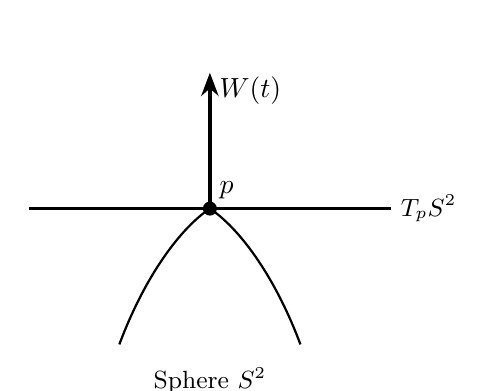
\begin{tikzpicture}[>=Stealth,scale=1.15]
		
		% Tangent plane
		\draw[thick] (-2,0)--(2,0);
		\node[right] at (2,0) {\small $T_pS^2$};
		
		% Point of tangency
		\fill (0,0) circle (2.2pt);
		\node[above right] at (0,0) {$p$};
		
		% Tangent vector
		\draw[->,very thick] (0,0)--(0,1.5);
		\node[right] at (0,1.3) {$W(t)$};
		
		% Sphere below
		\draw[thick] (-1,-1.5)
		.. controls (-0.7,-0.7) and (-0.3,-0.2) .. (0,0)
		.. controls (0.3,-0.2) and (0.7,-0.7) .. (1,-1.5);
		
		\node at (0,-1.9) {\small Sphere $S^2$};
		
	\end{tikzpicture}
\end{center}

For a rank-five vector bundle,

\[
\gamma(t)
\longrightarrow
E_{\gamma(t)},
\]

the picture becomes

\[
\boxed{
	\begin{array}{c}
		\textbf{Point } p\in S^2
		\\[3mm]
		\Downarrow
		\\[3mm]
		\text{Assign an ambient vector}
		\\[2mm]
		V(p)\in\mathbb{R}^{5}
		\\[2mm]
		V(p)=(w_1,w_2,w_3,w_4,w_5)
	\end{array}
}
\]

\[
\boxed{
	\begin{array}{c}
		\textbf{Tangent vector field}
		\\[3mm]
		W(p)\in T_pS^2
		\\[2mm]
		\dim(T_pS^2)=2
		\\[2mm]
		W(p)=a\,e_\theta+b\,e_\phi
	\end{array}
}
\]

The attached vector is no longer required to lie in the tangent plane.

%%%%%%%%%%%%%%%%%%%%%%%%%%%%%%%%%%%%%%%%%%%%%%%%%%%%%%

\subsection{Examples of Rank-Five Bundles}

Many geometric objects are vector bundles that are not tangent bundles.

Examples include

\begin{itemize}
	\item tangent bundle \(TM\),
	\item cotangent bundle \(T^*M\),
	\item tensor bundles,
	\item differential form bundles,
	\item spinor bundles,
	\item gauge bundles,
	\item arbitrary vector bundles of rank \(k\).
\end{itemize}

For any vector bundle

\[
E
\longrightarrow
M,
\]

a section along the curve satisfies

\[
\boxed{
	W(t)\in E_{\gamma(t)}.
}
\]

%%%%%%%%%%%%%%%%%%%%%%%%%%%%%%%%%%%%%%%%%%%%%%%%%%%%%%

\subsection{Comparison}

\begin{center}
	\begin{tabular}{|l|c|c|}
		\hline
		Object & Fiber at each point & Dimension\\
		\hline
		Tangent bundle \(TM\) & \(T_pM\) & \(\dim M\)\\
		Cotangent bundle \(T^*M\) & \(T_p^*M\) & \(\dim M\)\\
		Rank-5 vector bundle & \(E_p\cong\mathbb R^5\) & \(5\)\\
		Rank-\(k\) bundle & \(E_p\cong\mathbb R^k\) & \(k\)\\
		\hline
	\end{tabular}
\end{center}

%%%%%%%%%%%%%%%%%%%%%%%%%%%%%%%%%%%%%%%%%%%%%%%%%%%%%%

\subsection{Summary}

There are two fundamentally different kinds of vector fields.

\paragraph{Tangent vector field}

The vectors belong to the tangent spaces:

\[
\boxed{
	W(p)\in T_pM.
}
\]

Their dimension is always

\[
\boxed{
	\dim W=\dim M.
}
\]

%%%%%%%%%%%%%%%%%%%%%%%%%%%%%%%%%%%%%%%%%%%%%%%%%%%%%%

\paragraph{General bundle-valued field}

The vectors belong to another vector bundle:

\[
\boxed{
	W(p)\in E_p.
}
\]

The fiber dimension is determined by the bundle itself:

\[
\boxed{
	\dim E_p=k,
}
\]

which is completely independent of the dimension of the manifold.

For example, one may have a two-dimensional sphere together with a
rank-five vector bundle.

Then every point of the sphere carries an attached copy of

\[
\mathbb R^5,
\]

and one may assign a five-dimensional vector to every point.

Such a field is **not** a tangent vector field; rather, it is a section
of a rank-five vector bundle over the sphere.


\section{From Paths on the Sphere to Geodesics}

This chapter develops the central ideas of Riemannian geometry on the sphere in their
natural logical order. Beginning with a smooth path on the sphere, we introduce tangent
planes, vector fields, the Levi--Civita connection, parallel transport, and finally geodesics.
The sphere provides perhaps the simplest nontrivial example where all of these concepts
can be understood explicitly.

%%%%%%%%%%%%%%%%%%%%%%%%%%%%%%%%%%%%%%%%%%%%%%%%%%%%%%%%%%%%%%%%%%%%%%
\subsection{A Smooth Path on the Sphere}

Consider the unit sphere

\[
S^2=\{p\in\mathbb R^3:\|p\|=1\}.
\]

Let

\[
\gamma:I\rightarrow S^2
\]

be a smooth curve, where

\[
t\longmapsto\gamma(t).
\]

Since every point of the curve lies on the sphere,

\[
\|\gamma(t)\|^2=1.
\]

Differentiating gives

\[
\frac{d}{dt}\langle\gamma,\gamma\rangle
=
2\langle\gamma,\dot\gamma\rangle
=
0.
\]

Hence

\[
\boxed{\langle\gamma(t),\dot\gamma(t)\rangle=0.}
\]

Therefore,

\[
\boxed{\dot\gamma(t)\in T_{\gamma(t)}S^2.}
\]

The velocity vector is automatically tangent to the sphere.

Thus every smooth path immediately determines a tangent vector field,
namely its velocity.

%%%%%%%%%%%%%%%%%%%%%%%%%%%%%%%%%%%%%%%%%%%%%%%%%%%%%%%%%%%%%%%%%%%%%%
\subsection{The Tangent Plane Along the Path}

For every point

\[
p\in S^2
\]

the tangent plane is

\[
T_pS^2
=
\{v\in\mathbb R^3:\langle p,v\rangle=0\}.
\]

As the point moves,

\[
\gamma(t),
\]

its tangent plane also moves,

\[
T_{\gamma(t)}S^2.
\]

Consequently we obtain a continuously changing family of tangent planes

\[
T_{\gamma(t)}S^2,
\qquad
t\in I.
\]

It is important to distinguish three different objects.

\[
\gamma(t)
\]

is the point on the sphere.

\[
\dot\gamma(t)
\]

is the velocity of the path.

Finally,

\[
W(t)\in T_{\gamma(t)}S^2
\]

is an arbitrary tangent vector field along the curve.

In general,

\[
W(t)\neq\dot\gamma(t).
\]

The vector field may point in any direction inside the tangent plane.

%%%%%%%%%%%%%%%%%%%%%%%%%%%%%%%%%%%%%%%%%%%%%%%%%%%%%%%%%%%%%%%%%%%%%%
\subsection{A Path-Adapted Tangent Basis}

Assume that the curve is regular,

\[
\dot\gamma(t)\neq0.
\]

Its unit tangent vector is

\[
T(t)
=
\frac{\dot\gamma(t)}
{\|\dot\gamma(t)\|}.
\]

The outward unit normal of the sphere equals

\[
N_S(t)=\gamma(t).
\]

A second tangent vector may be defined by

\[
U(t)
=
N_S(t)\times T(t)
=
\gamma(t)\times T(t).
\]

Then

\[
\boxed{
	\{T(t),U(t)\}
}
\]

forms an orthonormal basis of the tangent plane.

Therefore,

\[
T_{\gamma(t)}S^2
=
\operatorname{span}\{T,U\}.
\]

Every tangent vector field can therefore be written as

\[
W(t)
=
a(t)T(t)+b(t)U(t).
\]

This basis is adapted to the motion of the curve and will later be compared
with the geographical east--north basis.

%%%%%%%%%%%%%%%%%%%%%%%%%%%%%%%%%%%%%%%%%%%%%%%%%%%%%%%%%%%%%%%%%%%%%%
\subsection{The Ordinary Derivative}

Because

\[
S^2\subset\mathbb R^3,
\]

every tangent vector may be regarded as an ordinary vector in Euclidean space,

\[
W(t)=
\begin{pmatrix}
	W^1(t)\\
	W^2(t)\\
	W^3(t)
\end{pmatrix}.
\]

Therefore,

\[
\dot W
=
\frac{dW}{dt}
\]

is computed exactly as in multivariable calculus.

However,

\[
W(t)\in T_{\gamma(t)}S^2
\]

does not imply

\[
\dot W(t)\in T_{\gamma(t)}S^2.
\]

The reason is that the tangent plane itself rotates while moving over the sphere.

The derivative therefore contains two different effects.

\begin{enumerate}
	\item
	Actual change of the vector inside the tangent plane.
	
	\item
	Apparent change caused by the rotation of the tangent plane itself.
\end{enumerate}

%%%%%%%%%%%%%%%%%%%%%%%%%%%%%%%%%%%%%%%%%%%%%%%%%%%%%%%%%%%%%%%%%%%%%%
\subsection{Tangential and Normal Components}

Every vector in $\mathbb R^3$ can be decomposed into tangent and normal parts,

\[
\dot W
=
(\dot W)^\top
+
(\dot W)^\perp.
\]

For the unit sphere the normal direction is

\[
\gamma(t).
\]

Hence

\[
(\dot W)^\perp
=
(\dot W\cdot\gamma)\gamma.
\]

Consequently,

\[
(\dot W)^\top
=
\dot W
-
(\dot W\cdot\gamma)\gamma.
\]

Only the tangential part describes intrinsic motion on the surface.

%%%%%%%%%%%%%%%%%%%%%%%%%%%%%%%%%%%%%%%%%%%%%%%%%%%%%%%%%%%%%%%%%%%%%%
\subsection{The Levi--Civita Connection}

The Levi--Civita derivative is defined by projecting the ordinary derivative
onto the tangent plane,

\[
\boxed{
	\nabla_{\dot\gamma}W
	=
	\operatorname{proj}_{T_{\gamma(t)}S^2}
	(\dot W).
}
\]

Using the projection formula,

\[
\boxed{
	\nabla_{\dot\gamma}W
	=
	\dot W
	-
	(\dot W\cdot\gamma)\gamma.
}
\]

Since

\[
W\cdot\gamma=0,
\]

differentiate to obtain

\[
\dot W\cdot\gamma
+
W\cdot\dot\gamma
=
0.
\]

Therefore,

\[
\dot W\cdot\gamma
=
-
W\cdot\dot\gamma.
\]

Substituting yields the equivalent intrinsic formula

\[
\boxed{
	\nabla_{\dot\gamma}W
	=
	\dot W
	+
	(W\cdot\dot\gamma)\gamma.
}
\]

For a sphere of radius $R$,

\[
\boxed{
	\nabla_{\dot\gamma}W
	=
	\dot W
	+
	\frac{W\cdot\dot\gamma}{R^2}\gamma.
}
\]

%%%%%%%%%%%%%%%%%%%%%%%%%%%%%%%%%%%%%%%%%%%%%%%%%%%%%%%%%%%%%%%%%%%%%%
\subsection{Parallel Transport}

A vector field is called parallel if

\[
\boxed{
	\nabla_{\dot\gamma}W=0.
}
\]

Using the previous formula,

\[
\boxed{
	\dot W
	=
	-
	(W\cdot\dot\gamma)\gamma.
}
\]

Notice carefully that

\[
\nabla_{\dot\gamma}W=0
\]

does not mean

\[
\dot W=0.
\]

Instead,

\[
\dot W
\]

may still be nonzero, but it is entirely normal to the sphere.

The vector is therefore allowed to rotate in the surrounding Euclidean space,
provided that it does not rotate intrinsically inside the tangent plane.

%%%%%%%%%%%%%%%%%%%%%%%%%%%%%%%%%%%%%%%%%%%%%%%%%%%%%%%%%%%%%%%%%%%%%%
\subsection{Preservation of Length and Angles}

Parallel transport preserves vector length.

Indeed,

\[
\frac{d}{dt}\|W\|^2
=
2\langle W,\nabla_{\dot\gamma}W\rangle.
\]

If

\[
\nabla_{\dot\gamma}W=0,
\]

then

\[
\boxed{
	\|W(t)\|
	=
	\text{constant}.
}
\]

Similarly, if

\[
\nabla_{\dot\gamma}W
=
0,
\qquad
\nabla_{\dot\gamma}Z
=
0,
\]

then

\[
\frac{d}{dt}
\langle W,Z\rangle
=
0.
\]

Hence parallel transport preserves both lengths and angles.

%%%%%%%%%%%%%%%%%%%%%%%%%%%%%%%%%%%%%%%%%%%%%%%%%%%%%%%%%%%%%%%%%%%%%%
\subsection{Geodesics}

The most important application of the Levi--Civita connection is the definition
of geodesics.

A smooth curve is called a geodesic if its own velocity vector is parallel
transported along the curve.

Thus

\[
\boxed{
	\nabla_{\dot\gamma}\dot\gamma
	=
	0.
}
\]

Therefore,

\[
\boxed{
	\text{A geodesic is a curve whose velocity remains parallel to itself.}
}
\]

%%%%%%%%%%%%%%%%%%%%%%%%%%%%%%%%%%%%%%%%%%%%%%%%%%%%%%%%%%%%%%%%%%%%%%
\subsection{The Geodesic Equation on the Sphere}

Substitute

\[
W=\dot\gamma
\]

into the Levi--Civita derivative:

\[
\nabla_{\dot\gamma}\dot\gamma
=
\ddot\gamma
+
(\dot\gamma\cdot\dot\gamma)\gamma.
\]

Therefore,

\[
\boxed{
	\ddot\gamma
	+
	\|\dot\gamma\|^2\gamma
	=
	0.
}
\]

If the parameter is arc length,

\[
\|\dot\gamma\|=1,
\]

then

\[
\boxed{
	\ddot\gamma
	=
	-
	\gamma.
}
\]

Thus the ordinary acceleration points entirely toward the center of the sphere.

There is no tangential acceleration.

%%%%%%%%%%%%%%%%%%%%%%%%%%%%%%%%%%%%%%%%%%%%%%%%%%%%%%%%%%%%%%%%%%%%%%
\subsection{Solution of the Geodesic Equation}

Suppose

\[
\gamma(0)=p,
\qquad
\dot\gamma(0)=v,
\]

where

\[
\|p\|=1,
\qquad
p\cdot v=0,
\qquad
\|v\|=1.
\]

The differential equation

\[
\ddot\gamma=-\gamma
\]

has solution

\[
\boxed{
	\gamma(t)
	=
	p\cos t
	+
	v\sin t.
}
\]

Since

\[
\gamma(t)
\in
\operatorname{span}\{p,v\},
\]

the entire curve lies in the two-dimensional plane generated by the initial
position and velocity.

The intersection of this plane with the sphere is a great circle.

Therefore,

\[
\boxed{
	\text{The geodesics of the sphere are precisely the great circles.}
}
\]

%%%%%%%%%%%%%%%%%%%%%%%%%%%%%%%%%%%%%%%%%%%%%%%%%%%%%%%%%%%%%%%%%%%%%%
\subsection{Great Circles and Latitude Circles}

Consider the equator,

\[
\gamma(t)
=
(\cos t,\sin t,0).
\]

Then

\[
\ddot\gamma
=
-
\gamma,
\]

so

\[
\nabla_{\dot\gamma}\dot\gamma
=
0.
\]

Hence the equator is a geodesic.

Now consider a latitude circle,

\[
\gamma(t)
=
(\cos\phi\cos t,
\cos\phi\sin t,
\sin\phi).
\]

Its velocity satisfies

\[
\|\dot\gamma\|^2
=
\cos^2\phi.
\]

The covariant acceleration becomes

\[
\nabla_{\dot\gamma}\dot\gamma
=
\ddot\gamma
+
\cos^2\phi\,\gamma.
\]

After simplification,

\[
\nabla_{\dot\gamma}\dot\gamma
=
\sin\phi\cos\phi
\begin{pmatrix}
	-\sin\phi\cos t\\
	-\sin\phi\sin t\\
	\cos\phi
\end{pmatrix}.
\]

This vanishes only when

\[
\phi=0.
\]

Therefore,

\[
\boxed{
	\text{Only the equator among the latitude circles is a geodesic.}
}
\]

%%%%%%%%%%%%%%%%%%%%%%%%%%%%%%%%%%%%%%%%%%%%%%%%%%%%%%%%%%%%%%%%%%%%%%
\subsection{Geodesic Curvature}

For every unit-speed curve,

\[
\ddot\gamma
=
-
\gamma
+
\nabla_TT.
\]

The term

\[
-\gamma
\]

represents the unavoidable normal curvature of the sphere.

The tangential component

\[
\nabla_TT
\]

measures how the curve bends inside the surface.

Its norm,

\[
\boxed{
	k_g
	=
	\|\nabla_TT\|,
}
\]

is called the geodesic curvature.

Consequently,

\[
\boxed{
	k_g=0
	\iff
	\gamma
	\text{ is a geodesic.}
}
\]

%%%%%%%%%%%%%%%%%%%%%%%%%%%%%%%%%%%%%%%%%%%%%%%%%%%%%%%%%%%%%%%%%%%%%%
\subsection{Logical Summary}

The concepts introduced in this chapter form the following chain:

\[
\boxed{
	\begin{aligned}
		\text{Sphere}
		&\longrightarrow
		\text{Path}
		\longrightarrow
		\text{Velocity}
		\longrightarrow
		\text{Tangent Plane}
		\\[1mm]
		&\longrightarrow
		\text{Vector Field}
		\longrightarrow
		\text{Ordinary Derivative}
		\longrightarrow
		\text{Projection}
		\\[1mm]
		&\longrightarrow
		\text{Levi--Civita Connection}
		\longrightarrow
		\text{Parallel Transport}
		\\[1mm]
		&\longrightarrow
		\text{Geodesics}
		\longrightarrow
		\text{Geodesic Curvature}.
	\end{aligned}
}
\]

This progression reveals the natural role of the Levi--Civita connection:
it provides the intrinsic notion of differentiation on curved manifolds,
makes parallel transport possible, and leads directly to the definition of geodesics.

\end{document}

